\documentclass[11pt]{article}
\usepackage[a4paper,left=19mm,right=19mm,top=19mm,bottom=19mm]{geometry}
\usepackage[T1]{fontenc}
\usepackage{lmodern,microtype,amsmath,amssymb,mathtools,booktabs,array}
\usepackage[most]{tcolorbox}
\usepackage{tikz,pgfplots,fancyhdr,enumitem,hyperref}
\usetikzlibrary{arrows.meta,positioning,calc,matrix,patterns}
\pgfplotsset{compat=1.18}
\definecolor{ink}{HTML}{182B3A}
\definecolor{teal}{HTML}{007F86}
\definecolor{orange}{HTML}{B96117}
\definecolor{purple}{HTML}{6A4C93}
\definecolor{blue}{HTML}{336699}
\definecolor{muted}{HTML}{5C6B78}
\definecolor{pale}{HTML}{F1F5F7}
\color{ink}
\hypersetup{colorlinks=true,linkcolor=teal,urlcolor=teal,pdftitle={Understanding the all-components IRMF bound},pdfauthor={IMF research project},bookmarksopen=true}
\setlength{\parindent}{0pt}
\setlength{\parskip}{5.5pt}
\setlength{\headheight}{14pt}
\setlength{\footskip}{22pt}
\emergencystretch=1.5em
\pagestyle{fancy}
\fancyhf{}
\fancyhead[L]{\sffamily\small\color{muted}IRMF / A visual proof guide}
\fancyhead[R]{\sffamily\small\color{muted}31 October 2026}
\fancyfoot[L]{\sffamily\scriptsize\color{muted}Leading fluctuation \textcolor{teal}{$\blacksquare$}\quad Remainder \textcolor{orange}{$\blacksquare$}\quad Population target \textcolor{purple}{$\blacksquare$}}
\fancyfoot[R]{\sffamily\small\thepage\,/\,12}
\renewcommand{\headrulewidth}{0.3pt}
\setlist[itemize]{leftmargin=16pt,itemsep=3pt,topsep=3pt}
\setlist[enumerate]{leftmargin=18pt,itemsep=3pt,topsep=3pt}
\newcommand{\E}{\mathbb E}
\newcommand{\Prb}{\mathbb P}
\newcommand{\norm}[1]{\lVert#1\rVert}
\newcommand{\al}{\alpha}
\newcommand{\eps}{\varepsilon}
\newcommand{\M}{\mathcal M}
\newcommand{\sub}[1]{\par\vspace{3pt}{\sffamily\bfseries\large #1}\par}
\newcommand{\captext}[1]{{\small\color{muted}#1}\par}
\newcommand{\chapterpage}[3]{\clearpage\phantomsection\pdfbookmark[0]{#2}{page#1}{\sffamily\color{teal}\small #1\quad /\quad #3}\par\vspace{3pt}{\sffamily\bfseries\LARGE #2}\par\vspace{3pt}}
\newtcolorbox{idea}[1][]{enhanced,colback=teal!5,colframe=teal!70,boxrule=.55pt,arc=1.3mm,left=9pt,right=9pt,top=7pt,bottom=7pt,before skip=8pt,after skip=8pt,#1}
\newtcolorbox{result}[1][]{enhanced,colback=orange!5,colframe=orange!75,boxrule=.55pt,arc=1.3mm,left=9pt,right=9pt,top=7pt,bottom=7pt,before skip=8pt,after skip=8pt,#1}
\newtcolorbox{targetbox}[1][]{enhanced,colback=purple!4,colframe=purple!65,boxrule=.55pt,arc=1.3mm,left=9pt,right=9pt,top=7pt,bottom=7pt,before skip=8pt,after skip=8pt,#1}
\tikzset{box/.style={draw=teal!65,fill=teal!5,rounded corners=2pt,align=center,minimum height=10mm,inner sep=5pt,font=\small}, flow/.style={-{Stealth[length=2mm]},thick,draw=muted}}
\pgfplotsset{guide/.style={width=\linewidth,height=54mm,axis lines=left,tick label style={font=\scriptsize},label style={font=\small},title style={font=\small\bfseries},legend style={font=\scriptsize,draw=none,fill=none},grid=major,grid style={gray!13},every axis plot/.append style={thick},mark size=1.6pt}}
% Generated by build_visual_guide.py; do not edit by hand.
\def\freqOne{(0,1) (1,0.88363569) (2,0.60793024) (3,0.32753126) (4,0.15198856) (5,0.084891068) (6,0.067554916) (7,0.054147604) (8,0.038003141) (9,0.027905312) (10,0.024324891) (11,0.021267686) (12,0.016894731) (13,0.01369207) (14,0.012414579) (15,0.011274195) (16,0.009506789) (17,0.0081070584) (18,0.0075132179) (19,0.0069696837) (20,0.0060872286) (21,0.0053548818) (22,0.0050321583) (23,0.004732008) (24,0.0042296913) (25,0.0037996365) (26,0.0036051836) (27,0.003422311) (28,0.0031096564) (29,0.0028359654) (30,0.0027098908) (31,0.0025903524) (32,0.0023827124) (33,0.0021978963) (34,0.0021115554) (35,0.0020291776) (36,0.0018843236) (37,0.0017537119) (38,0.0016920179) (39,0.0016328644) (40,0.0015278309)}
\def\freqThree{(0,0) (1,0.0067752872) (2,0.07626623) (3,0.21857993) (4,0.32530309) (5,0.32893661) (6,0.2666015) (7,0.19363434) (8,0.13577308) (9,0.098441704) (10,0.078468687) (11,0.069291054) (12,0.064314294) (13,0.059098509) (14,0.052184585) (15,0.04431196) (16,0.036915502) (17,0.031116612) (18,0.027322444) (19,0.02518845) (20,0.023902957) (21,0.022646926) (22,0.020966036) (23,0.018875787) (24,0.016709962) (25,0.01486232) (26,0.013566017) (27,0.012796422) (28,0.012322053) (29,0.011855239) (30,0.011208138) (31,0.01036755) (32,0.0094616321) (33,0.0086610522) (34,0.0080796883) (35,0.00772201) (36,0.0074951385) (37,0.0072708185) (38,0.0069576498) (39,0.0065424872) (40,0.0060834423)}
\def\freqFive{(0,0) (1,3.1982263e-06) (2,0.00057861687) (3,0.0084721298) (4,0.040479546) (5,0.10232305) (6,0.17718741) (7,0.2446491) (8,0.29097263) (9,0.31041778) (10,0.30642227) (11,0.28667094) (12,0.25757172) (13,0.22401592) (14,0.19051527) (15,0.16039688) (16,0.13502169) (17,0.11446054) (18,0.09843711) (19,0.086565529) (20,0.078232716) (21,0.072627575) (22,0.068901571) (23,0.066275623) (24,0.064078948) (25,0.06180438) (26,0.059169095) (27,0.056096069) (28,0.052628979) (29,0.048875695) (30,0.044997655) (31,0.041186662) (32,0.037618396) (33,0.034423465) (34,0.031685964) (35,0.029445108) (36,0.027691831) (37,0.026372203) (38,0.025400386) (39,0.024672025) (40,0.024075416)}
\def\freqSeven{(0,0) (1,9.2726048e-11) (2,2.6863136e-07) (3,1.9941457e-05) (4,0.00030181086) (5,0.001868645) (6,0.006740048) (7,0.017344464) (8,0.035463929) (9,0.061187024) (10,0.093121034) (11,0.12922798) (12,0.16674703) (13,0.20241108) (14,0.23388341) (15,0.26029593) (16,0.28107862) (17,0.29534162) (18,0.30272078) (19,0.30393813) (20,0.3002088) (21,0.29259283) (22,0.28194375) (23,0.26897493) (24,0.25422687) (25,0.23819118) (26,0.22149641) (27,0.20483079) (28,0.18870784) (29,0.17341384) (30,0.15913274) (31,0.14600983) (32,0.13411168) (33,0.12341807) (34,0.11387882) (35,0.10545232) (36,0.098096514) (37,0.091757637) (38,0.086373911) (39,0.081871045) (40,0.078150888)}
\def\freqNine{(0,-0) (1,1.6780098e-16) (2,7.7802529e-12) (3,2.9252902e-09) (4,1.4002381e-07) (5,2.1185064e-06) (6,1.5863181e-05) (7,7.5733328e-05) (8,0.00026461552) (9,0.00073276847) (10,0.0017037314) (11,0.0034710191) (12,0.0063630229) (13,0.010676452) (14,0.016659856) (15,0.024544055) (16,0.034482587) (17,0.04643248) (18,0.0601835) (19,0.075512652) (20,0.092227244) (21,0.11009121) (22,0.12880359) (23,0.14800592) (24,0.1672451) (25,0.18602099) (26,0.20396918) (27,0.22093813) (28,0.23684204) (29,0.25153754) (30,0.26489211) (31,0.27685442) (32,0.28737404) (33,0.29632571) (34,0.30357719) (35,0.30908321) (36,0.31288529) (37,0.31508372) (38,0.3158381) (39,0.3153327) (40,0.31370252)}
\def\residualNorm{(1,1) (2,1.9880001) (3,2.0939665) (4,2.1086554) (5,2.0975447) (6,2.0791528) (7,2.0530184) (8,2.0139476) (9,1.9596558)}
\def\componentNorm{(1,1) (2,0.49697422) (3,0.44700533) (4,0.43471534) (5,0.42402247) (6,0.41446117) (7,0.41478555) (8,0.41010739) (9,0.43164752)}
\def\mcGaussian{(1,1.3169929) (2,2.4271377) (3,3.0292014) (4,3.5196279) (5,4.1809421) (6,5.2368592) (7,6.1898577) (8,7.6465021) (9,10.368975)}
\def\mcContaminated{(1,2.9369566) (2,5.6868208) (3,7.4246294) (4,9.5699352) (5,12.834068) (6,17.706378) (7,22.968877) (8,31.27404) (9,41.570744)}

\begin{document}

\chapterpage{01}{Why later components stay accurate}{The question}
IRMF fits a local level, subtracts it, and repeats with a smaller window.
The first component uses the observed data. Every later component uses a
residual that already contains fitting errors. The proof has to track those errors.

\begin{center}
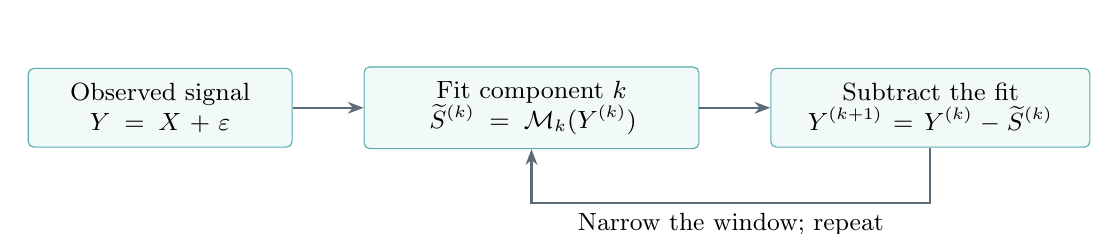
\begin{tikzpicture}[node distance=9mm]
\node[box,text width=30mm] (y) {Observed signal\\$Y=X+\eps$};
\node[box,right=of y,text width=39mm] (fit) {Fit component $k$\\$\widetilde S^{(k)}=\M_k(Y^{(k)})$};
\node[box,right=of fit,text width=37mm] (res) {Subtract the fit\\$Y^{(k+1)}=Y^{(k)}-\widetilde S^{(k)}$};
\draw[flow] (y)--(fit);
\draw[flow] (fit)--(res);
\draw[flow] (res.south)--++(0,-7mm)-|node[pos=.25,below,font=\small]{Narrow the window; repeat} (fit.south);
\end{tikzpicture}
\end{center}
\vspace{5mm}
The goal is a bound at each component's \emph{own} scale. Write
\[
 \al_k=\max_{t,u}a_{tu}^{(k)},\qquad z=x+\log(10nK).
\]
The $a_{tu}^{(k)}$ are nonnegative local weights with row sum one.
For a uniform window of $m_k$ observations, $\al_k=1/m_k$.
More generally, $1/\al_k$ is a useful window-size proxy.
The number $x$ sets the failure probability $e^{-x}$; the logarithm pays
for checking all $n$ positions and $K$ stages.

\begin{idea}
\textbf{The form of the result}
\[
 \norm{\widetilde S^{(k)}-S_\phi^{(k)}}_\infty
 \le \underbrace{A_\Lambda\sqrt{z\al_k}}_{\text{leading fluctuation}}
     +\underbrace{C_Qz\al_k}_{\text{nonlinear remainder}}.
\]
The sup norm is the largest absolute error over the observed time grid.
The constants can stay independent of the stage. A separate correction
transfers this bound to the paper's population target.
\end{idea}

\sub{What the two scales mean}
If $z\al_k=0.01$, their bare sizes are $0.1$ and $0.01$.
If the window size is halved, the leading scale grows by $\sqrt2$ and the
second-order scale doubles. These are scale comparisons; the constants
still decide whether a finite sample is covered.

\begin{center}
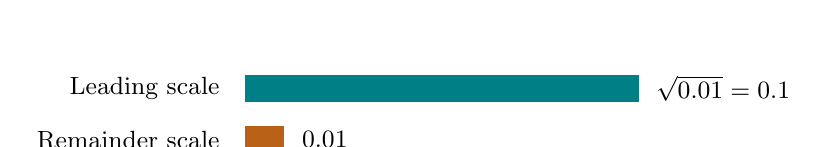
\begin{tikzpicture}[x=1cm,y=1cm]
\node[anchor=east,font=\small] at (3,1) {Leading scale};
\node[anchor=east,font=\small] at (3,.35) {Remainder scale};
\fill[teal] (3.2,.83) rectangle (8.2,1.17);
\fill[orange] (3.2,.18) rectangle (3.7,.52);
\node[anchor=west,font=\small] at (8.3,1) {$\sqrt{0.01}=0.1$};
\node[anchor=west,font=\small] at (3.8,.35) {$0.01$};
\end{tikzpicture}
\end{center}
\begin{result}
\textbf{Scope of this guide.} The propagation remainder and induction are
proved under added curvature-dispersion and sample-size conditions.
The paper-target comparison also uses a fourth noise moment and tail
conditions. The original statement without these restrictions remains open.
\end{result}
\captext{Route through the proof: linear stability $\to$ local expansion $\to$
exact recursion $\to$ propagation $\to$ induction $\to$ target correction.}

\chapterpage{02}{Which target are we estimating?}{Three paths}
The same symbol ``component'' can hide different targets. Fix a deterministic
signal $X$ and independent, identically distributed noises $\eps_u$.
The local fitting map is
\[
 \M_k(y)_t=\arg\min_s\sum_u a_{tu}^{(k)}\rho_H(y_u-s).
\]
The smooth absolute loss has bounded score $|\rho_H'|\le1$ and positive
curvature. Define its noise-averaged version by
\[
 \phi(c)=\E\{\rho_H(c+\eps)-\rho_H(\eps)\}.
\]
Subtracting $\rho_H(\eps)$ makes this expectation finite even when the
noise has no first moment. It does not change the score or minimizer.

\begin{center}
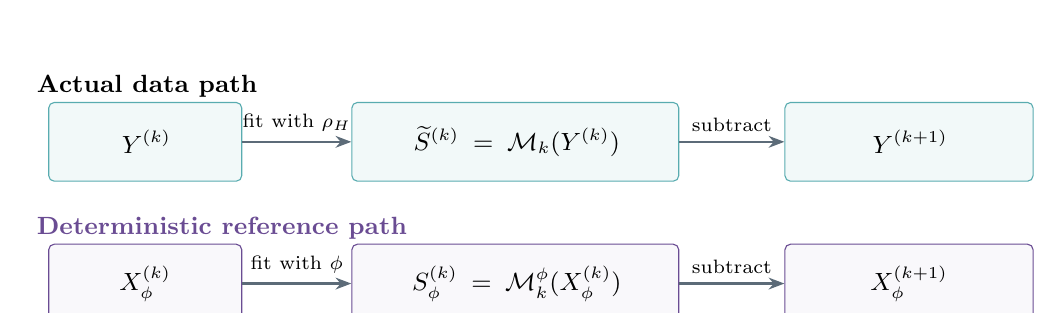
\begin{tikzpicture}[x=1cm,y=1cm]
\node[anchor=west,font=\small\bfseries] at (0,3.7) {Actual data path};
\node[box,text width=21mm] (a) at (1.5,3) {$Y^{(k)}$};
\node[box,text width=38mm] (b) at (6.2,3) {$\widetilde S^{(k)}=\M_k(Y^{(k)})$};
\node[box,text width=28mm] (c) at (11.2,3) {$Y^{(k+1)}$};
\draw[flow] (a)--node[above,font=\scriptsize]{fit with $\rho_H$}(b);
\draw[flow] (b)--node[above,font=\scriptsize]{subtract}(c);
\node[anchor=west,font=\small\bfseries,text=purple] at (0,1.9) {Deterministic reference path};
\node[box,draw=purple,fill=purple!4,text width=21mm] (d) at (1.5,1.2) {$X_\phi^{(k)}$};
\node[box,draw=purple,fill=purple!4,text width=38mm] (e) at (6.2,1.2) {$S_\phi^{(k)}=\M_k^{\phi}(X_\phi^{(k)})$};
\node[box,draw=purple,fill=purple!4,text width=28mm] (f) at (11.2,1.2) {$X_\phi^{(k+1)}$};
\draw[flow] (d)--node[above,font=\scriptsize]{fit with $\phi$}(e);
\draw[flow] (e)--node[above,font=\scriptsize]{subtract}(f);
\end{tikzpicture}
\end{center}
Here $Y^{(1)}=X+\eps$ and $X_\phi^{(1)}=X$. The superscript $\phi$
on the smoother means replace $\rho_H$ by $\phi$ in the minimization.

\begin{targetbox}
\textbf{The paper's target uses the law of the actual residual}
\[
 S_{{\rm pdf},t}^{(k)}
 =\arg\min_s\sum_u a_{tu}^{(k)}\E\rho_H(Y_u^{(k)}-s).
\]
This is a deterministic target, but its input law comes from the noisy
recursion. At stage one it equals $S_\phi^{(1)}$. At later stages that
identity needs proof and is generally replaced by a small target correction.
\end{targetbox}

\sub{Why introduce the $\phi$ path?}
Define the component error $e_k$ and accumulated error $E_k$ by
\[
 e_k=\widetilde S^{(k)}-S_\phi^{(k)},\qquad
 E_k=\sum_{j<k}e_j.
\]
Subtracting the two recursions gives the exact identity
\begin{idea}
\[
 Y^{(k)}=\underbrace{X_\phi^{(k)}+\eps}_{\text{deterministic signal + original noise}}
           -\underbrace{E_k}_{\text{earlier fitting errors}}.
\]
We can expand a single pass at $X_\phi^{(k)}+\eps$, then study the input
perturbation $-E_k$. All stages reuse the same original noise vector.
\end{idea}
\captext{A clean-data fit with the original loss $\rho_H$ is another reference.
It is not automatically either of the population targets above.}

\chapterpage{03}{Why products need their own bound}{Linear stability}
For a linear smoother $W_k$, the residual operator is $I-W_k$.
A single factor can have sup norm nearly two. Multiplying those norm
bounds gives $2^{k-1}$, which discards cancellation between stages.
For periodic convolution, Fourier coordinates expose that cancellation:
\[
 \widehat T_k(\omega)=\widehat W_k(\omega)
       \prod_{j<k}\{1-\widehat W_j(\omega)\}.
\]
Earlier stages suppress low frequencies. The current smoother suppresses
high frequencies. Their product selects an overlapping frequency band.

\begin{center}
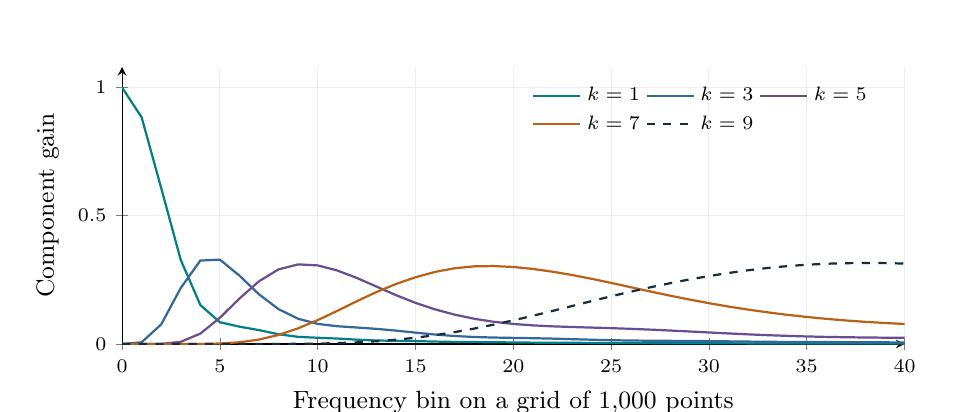
\begin{tikzpicture}
\begin{axis}[guide,width=.95\linewidth,height=51mm,xmin=0,xmax=40,ymin=0,ymax=1.08,xlabel={Frequency bin on a grid of 1,000 points},ylabel={Component gain},legend pos=north east,legend columns=3]
\addplot[teal] coordinates {\freqOne};\addlegendentry{$k=1$}
\addplot[blue] coordinates {\freqThree};\addlegendentry{$k=3$}
\addplot[purple] coordinates {\freqFive};\addlegendentry{$k=5$}
\addplot[orange] coordinates {\freqSeven};\addlegendentry{$k=7$}
\addplot[ink,dashed] coordinates {\freqNine};\addlegendentry{$k=9$}
\end{axis}
\end{tikzpicture}
\end{center}
\captext{Calculated linear transfer functions for normalized $(1-|u|)_+^2$ weights.\\
Window sizes: $501,355,251,177,125,89,63,45,31$.}

\begin{center}
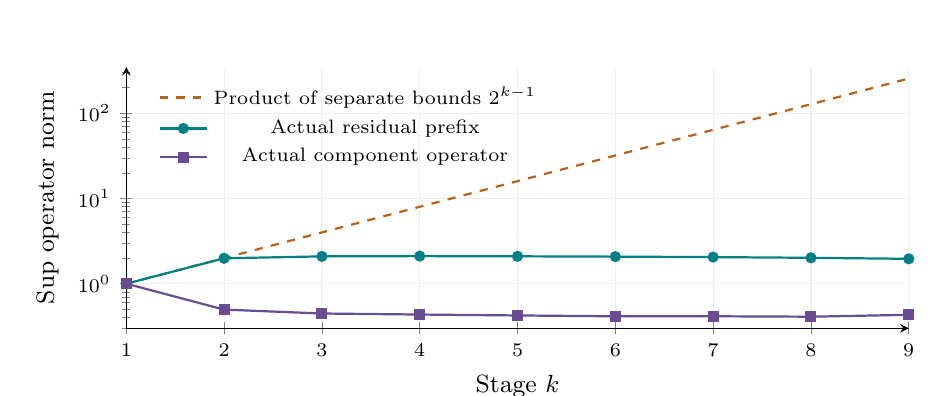
\begin{tikzpicture}
\begin{semilogyaxis}[guide,width=.95\linewidth,height=49mm,xmin=1,xmax=9,ymin=.3,ymax=350,xtick={1,...,9},xlabel={Stage $k$},ylabel={Sup operator norm},legend pos=north west]
\addplot[orange,dashed,domain=1:9,samples=9] {2^(x-1)};\addlegendentry{Product of separate bounds $2^{k-1}$}
\addplot[teal,mark=*] coordinates {\residualNorm};\addlegendentry{Actual residual prefix}
\addplot[purple,mark=square*] coordinates {\componentNorm};\addlegendentry{Actual component operator}
\end{semilogyaxis}
\end{tikzpicture}
\end{center}
\captext{These are finite-design calculations, not uniform kernel theorems.
Frequency control alone gives an $\ell_2$ bound; an $\ell_\infty$ proof also
controls the absolute mass of the inverse Fourier kernel.}

\begin{idea}
\textbf{What the nonlinear proof actually needs}
\[
 B_{m:l}=(I-V_m)\cdots(I-V_l),\qquad
 \norm{B_{m:l}}_\infty\le C_B
 \quad\text{for every interval }l\le m.
\]
The $V_k$ are population weights introduced next. They need not commute.
The theorem assumes this bound for the actual ordered products. The earlier
Fourier and perturbation lemmas provide one route to establishing it.
\end{idea}

\chapterpage{04}{One robust fit is nearly linear}{The Fisher expansion}
Fix stage $k$ and position $t$. For this page suppress those indices.
Let $S_\phi$ be the population fit and $c_u=X_{\phi,u}-S_\phi$.
The empirical score at that target is random, while its mean is zero:
\[
 q=\sum_u a_u\rho'(c_u+\eps_u),\qquad \E q=0,\qquad
 f=\sum_u a_u\E\rho''(c_u+\eps_u)\ge\lambda>0.
\]
Moving the fitted level by $h$ decreases the score at rate approximately
$f$. Its zero is therefore near $h=q/f$.

\begin{center}
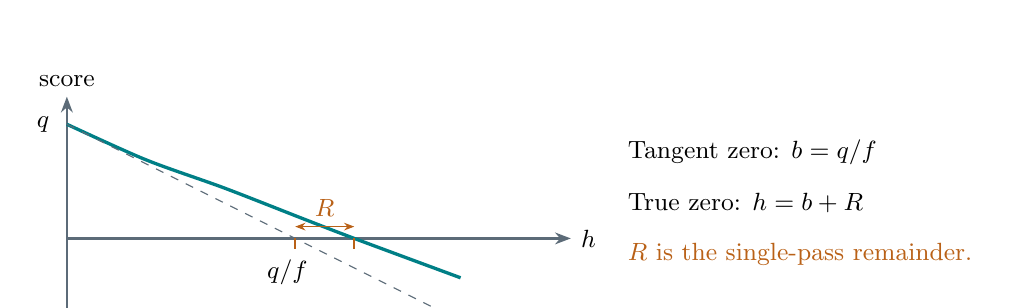
\begin{tikzpicture}[x=1cm,y=1cm]
\draw[flow] (0,0)--(6.4,0) node[right,font=\small] {$h$};
\draw[flow] (0,-1)--(0,1.8) node[above,font=\small] {score};
\draw[teal,very thick] plot[smooth] coordinates{(0,1.45)(1,1.00)(2,.64)(3,.25)(3.65,0)(5,-.5)};
\draw[muted,dashed] (0,1.45)--(4.8,-.95);
\node[anchor=east,font=\small] at (-.1,1.45) {$q$};
\draw[orange,thick] (2.9,0)--(2.9,-.14);
\node[below,font=\small] at (2.8,-.15) {$q/f$};
\draw[orange,thick] (3.65,0)--(3.65,-.14);
\draw[orange,{Stealth[length=1.3mm]}-{Stealth[length=1.3mm]}] (2.9,.15)--node[above,font=\small] {$R$}(3.65,.15);
\node[font=\small,anchor=west] at (7,1.1) {Tangent zero: $b=q/f$};
\node[font=\small,anchor=west] at (7,.45) {True zero: $h=b+R$};
\node[font=\small,anchor=west,text=orange] at (7,-.2) {$R$ is the single-pass remainder.};
\end{tikzpicture}
\end{center}
\captext{Schematic score curve. The proof controls the distance between the
tangent zero and the actual zero.}

For the smoothed absolute loss,
\[
 |\rho'|\le1,\quad 0<\rho''\le L_2=\frac{\sqrt{2/\pi}}H,\quad
 |\rho'''|\le L_3=\frac{\sqrt{2/\pi}e^{-1/2}}{H^2}.
\]
Write $u=c_u^*\sqrt{z\al_k}$ and $v=L_2c_v^*\sqrt{z\al_k}$, where
$c_u^*=\sqrt2+2/3$ and $c_v^*=\sqrt2+1/3$.
Concentration gives $|q|\le u$ and empirical curvature error at most $v$.
If $v\le\lambda/4$ and $u\le\lambda^2/(8L_3)$, the curvature stays at
least $\lambda/2$ within $|h|\le2u/\lambda$. The score crosses zero there.
Taylor's formula then gives
\begin{result}
\[
 |R|\le\frac{2uv}{\lambda^2}+\frac{2L_3u^2}{\lambda^3}
       =A_Rz\al_k,\qquad
 A_R=\frac{2L_2c_u^*c_v^*}{\lambda^2}
          +\frac{2L_3(c_u^*)^2}{\lambda^3}.
\]
The remainder is quadratic in the fluctuation scale.
\end{result}

\sub{The population weights}
Changing the input signal moves the population fit with weights
\[
 V_k[t,u]=\frac{a_{tu}^{(k)}\E\rho''(c_{tu}^{(k)}+\eps_u)}{f_{kt}}.
\]
They are nonnegative and sum to one. Observations in regions of low
expected curvature receive less influence. $V_k$ is a deterministic
population Jacobian. It is generally \emph{not} the expectation of the
random Jacobian of the empirical fit, whose denominator is random.

\chapterpage{05}{Separate the error before bounding it}{Exact bookkeeping}
The single-pass remainder $R_k$ describes fitting $X_\phi^{(k)}+\eps$.
The propagation remainder $\Phi_k$ describes changing that input by $-E_k$:
\[
 \Phi_k=\M_k(X_\phi^{(k)}+\eps)-\M_k(Y^{(k)})-V_kE_k.
\]
Substitution, with no approximation, yields
\begin{idea}
\[
 e_k=b_k+R_k-\Phi_k-V_kE_k,\qquad
 E_{k+1}=(I-V_k)E_k+b_k+R_k-\Phi_k.
\]
The term $-V_kE_k$ is the first-order response to all earlier errors.
It belongs in the leading recursion.
\end{idea}

Split accumulated error into a leading part and a remainder:
\begin{center}
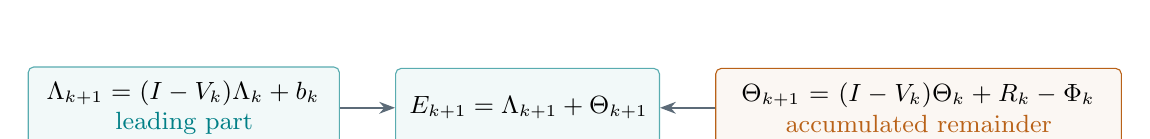
\begin{tikzpicture}[node distance=7mm]
\node[box,text width=36mm] (l) {$\Lambda_{k+1}=(I-V_k)\Lambda_k+b_k$\\\textcolor{teal}{leading part}};
\node[box,right=of l,text width=30mm] (e) {$E_{k+1}=\Lambda_{k+1}+\Theta_{k+1}$};
\node[box,draw=orange,fill=orange!5,right=of e,text width=48mm] (q) {$\Theta_{k+1}=(I-V_k)\Theta_k+R_k-\Phi_k$\\\textcolor{orange}{accumulated remainder}};
\draw[flow] (l)--(e);\draw[flow] (q)--(e);
\end{tikzpicture}
\end{center}
Start with $E_1=\Lambda_1=\Theta_1=0$. For an individual component,
\[
 \underbrace{e_k}_{\text{component error}}
 =\underbrace{b_k-V_k\Lambda_k}_{L_k}
  +\underbrace{\Theta_{k+1}-\Theta_k}_{Q_k}.
\]
Notice the distinction. $\Theta_k$ accumulates earlier nonlinear errors;
$Q_k$ is the nonlinear error in component $k$.

\sub{Check the first two stages by hand}
\begin{align*}
 e_1&=b_1+R_1,\\
 e_2&=\underbrace{b_2-V_2b_1}_{L_2}
       +\underbrace{R_2-V_2R_1-\Phi_2}_{Q_2}.
\end{align*}
Here $L_2$ in the second line means the stage-two leading vector;
the loss-curvature constant also denoted $L_2$ is a scalar.
Even the second component contains the same noise through both $b_1$ and $b_2$.

\sub{Unroll first, then take norms}
With $B_{m:l}=(I-V_m)\cdots(I-V_l)$ and empty product $I$,
\begin{align*}
 \Lambda_k&=\sum_{j<k}B_{k-1:j+1}b_j,\\
 \Theta_k&=\sum_{j<k}B_{k-1:j+1}(R_j-\Phi_j).
\end{align*}
These formulas retain the bounded full products. Estimating the recursion
one factor at a time would reintroduce the artificial exponential growth
from page 3. Order matters: in general, $V_iV_j\ne V_jV_i$.

\begin{result}
\textbf{The remaining task is precise.} Prove $\Theta_{k+1}=O(z\al_k)$
uniformly in $k$. Then $Q_k=\Theta_{k+1}-\Theta_k$ has the same order,
and concentration controls $L_k$.
\end{result}

\chapterpage{06}{Use independence in the right direction}{Leading concentration}
The vectors $b_1,b_2,\ldots$ are dependent. Each is computed from the same
$\eps_1,\ldots,\eps_n$. To apply concentration, collect every contribution
from observation $u$ into one summand.

\begin{center}
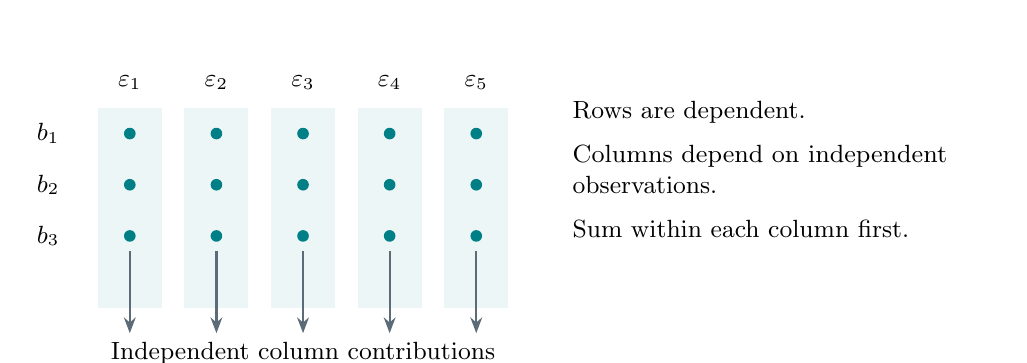
\begin{tikzpicture}[x=1.1cm,y=.65cm]
\foreach \u in {1,2,3,4,5} {
 \fill[teal!7] (\u-.37,-.4) rectangle (\u+.37,3.5);
 \node[font=\small] at (\u,4) {$\eps_{\u}$};
 \foreach \j in {1,2,3} {\fill[teal] (\u,\j) circle (2.1pt);}
 \draw[flow] (\u,.7)--(\u,-.9);
}
\foreach \j/\label in {3/{b_1},2/{b_2},1/{b_3}} {
 \node[anchor=east,font=\small] at (.3,\j) {$\label$};
}
\node[anchor=west,font=\small,text width=53mm] at (6,2.3) {Rows are dependent.\\[5pt]Columns depend on independent observations.\\[5pt]Sum within each column first.};
\node[font=\small] at (3,-1.3) {Independent column contributions};
\end{tikzpicture}
\end{center}

\sub{Why earlier stages do not add a factor $K$}
Assume the schedule satisfies
\[
 \al_j\le C_\al\al_k a^{-(k-j)}\quad(j\le k),\qquad a>1.
\]
Older stages have wider windows and smaller maximum weights.
The relevant sums are geometric:
\[
 \sum_{j\le k}\al_j\le s_1\al_k,\quad
 \sum_{j\le k}\sqrt{\al_j}\le s_2\sqrt{\al_k},\quad
 s_1=\frac{C_\al}{1-a^{-1}},\quad
 s_2=\frac{\sqrt{C_\al}}{1-a^{-1/2}}.
\]
For each observation, the score is bounded. Transferring it through a
matrix of norm at most $C_B$ gives a variance bound proportional to
$(C_B/\lambda)^2s_2^2\al_k$ and a maximum summand bound proportional to
$(2C_B/\lambda)s_1\al_k$. Bernstein's inequality gives
\begin{idea}
For $z\max_j\al_j\le1$, on one simultaneous event,
\[
 \norm{L_k}_\infty\le A_\Lambda\sqrt{z\al_k},\qquad
 \norm{\Lambda_k}_\infty\le A_\Lambda\sqrt{z\al_{k-1}},
 \quad
 A_\Lambda=\frac{C_B}{\lambda}
     \left(\sqrt2s_2+\frac23s_1\right).
\]
The second bound starts at $k=2$; $\Lambda_1=0$.
\end{idea}

\sub{One event for the entire proof}
The score, curvature, leading-term and quadratic-statistic bounds have a
total failure probability at most $10nKe^{-z}$. Choosing
$z=x+\log(10nK)$ makes that $e^{-x}$.
The event is fixed before induction. No step conditions on earlier
successes or treats a later residual as fresh independent noise.

\chapterpage{07}{The propagation remainder has four pieces}{The missing local estimate}
Set $y=X_\phi^{(k)}+\eps$, suppress $k$, and write $J(s)=D\M_k(y-sE)$.
Define curvature at the population target and its fluctuation by
\[
 g_u=\rho''(c_{tu}+\eps_u),\quad
 \overline M[t,u]=\frac{a_{tu}g_u}{f_t}=V[t,u]+Z[t,u].
\]
The fundamental theorem of calculus gives an exact split:
\begin{result}
\begin{align*}
 \Phi={}&\underbrace{\int_0^1[J(s)-J(0)]E\,ds}_{\text{1. Jacobian changes along the path}}\\
 &+\underbrace{[J(0)-\overline M]E}_{\text{2. fitted location and denominator change}}\\
 &+\underbrace{Z\Lambda}_{\text{3. curvature fluctuation times leading error}}\\
 &+\underbrace{Z\Theta}_{\text{4. feedback from the unknown remainder}}.
\end{align*}
\end{result}

\sub{1. Control the path using curvature at its start}
The smoother is monotone and translation equivariant, so
$\norm{\M(w)-\M(v)}_\infty\le\norm{w-v}_\infty$.
Each residual inside the loss changes by at most $2s\norm E_\infty$.
The Jacobian row is a normalized positive vector of curvature weights.
For positive-mass vectors $p,q\ge0$,
\[
 \left\|\frac p{\sum p}-\frac q{\sum q}\right\|_1
       \le\frac{2\norm{p-q}_1}{\sum q}.
\]
Choose $q$ at $s=0$, where page 4 gives curvature at least $\lambda/2$.
Thus $\norm{J(s)-J(0)}_\infty\le8L_3s\norm E_\infty/\lambda$.
Integrating gives $(4L_3/\lambda)\norm E_\infty^2$.
We only need positivity at the other points on the path.

\sub{2. Compare the fitted and population locations}
The fitted location moves by at most $2u/\lambda$.
The target curvature fluctuates by at most $v$.
Changing the numerator and its normalization therefore gives
\[
 \norm{J(0)-\overline M}_\infty
 \le C_{\rm loc}\sqrt{z\al_k},\qquad
 C_{\rm loc}=\frac{L_2c_v^*}{\lambda}+\frac{4L_3c_u^*}{\lambda^2}.
\]

\begin{idea}
Combining the four pieces,
\[
\begin{split}
 \norm{\Phi_k}_\infty\le{}&\frac{4L_3}{\lambda}\norm{E_k}_\infty^2
       +C_{\rm loc}\sqrt{z\al_k}\norm{E_k}_\infty\\
       &+\norm{Z_k\Lambda_k}_\infty
       +\norm{Z_k}_\infty\norm{\Theta_k}_\infty.
\end{split}
\]
Piece 3 needs cancellation. Piece 4 needs a coefficient small enough to
close the induction. A crude norm bound treats them too similarly.
\end{idea}

\chapterpage{08}{The difficult product is a quadratic statistic}{Cancellation by observation}
Write the accumulated leading error as a sum by noise coordinate:
\[
 \Lambda_k(u)=\sum_v\gamma_{uv}(\eps_v),\qquad \E\gamma_{uv}=0.
\]
For a fixed output position,
$(Z_k\Lambda_k)_t=\sum_{u,v}Z_k[t,u]\gamma_{uv}(\eps_v)$.
The two factors are independent only when $u\ne v$.

\begin{center}
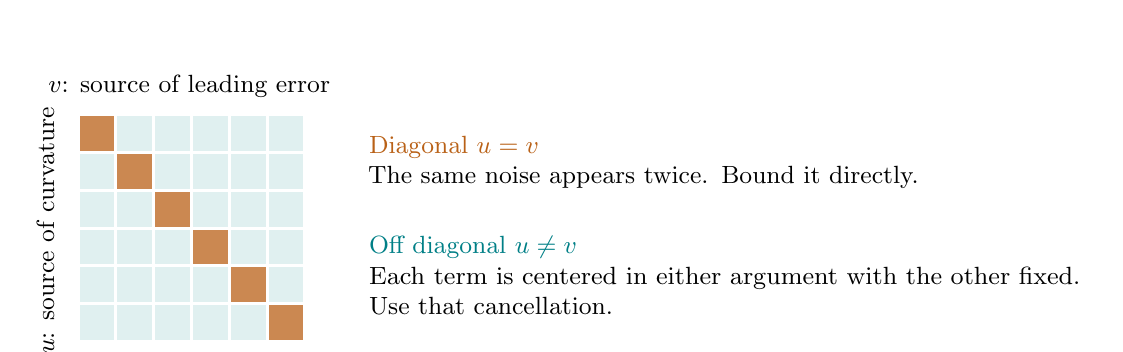
\begin{tikzpicture}[x=.48cm,y=.48cm]
\foreach \u in {0,...,5}{\foreach \v in {0,...,5}{
 \fill[teal!12] (\u,\v) rectangle ++(.92,.92);
}}
\foreach \u in {0,...,5}{\fill[orange!75] (\u,5-\u) rectangle ++(.92,.92);}
\node[font=\small] at (2.9,6.7) {$v$: source of leading error};
\node[rotate=90,font=\small] at (-.9,2.9) {$u$: source of curvature};
\node[anchor=west,font=\small,text width=91mm] at (7.4,4.7) {\textcolor{orange}{Diagonal $u=v$}\\The same noise appears twice. Bound it directly.};
\node[anchor=west,font=\small,text width=91mm] at (7.4,1.7) {\textcolor{teal}{Off diagonal $u\ne v$}\\Each term is centered in either argument with the other fixed. Use that cancellation.};
\end{tikzpicture}
\end{center}
Put $b_0=L_2/\lambda$, $G_\infty=2C_Bs_1/\lambda$ and
$G_2=2C_Bs_2/\lambda$. A deterministic envelope $|\gamma_{uv}|\le\Gamma_{uv}$
satisfies
\[
 \max_{u,v}\Gamma_{uv}\le G_\infty\al_{k-1},\qquad
 \max_u\left(\sum_v\Gamma_{uv}^2\right)^{1/2}
      \le G_2\sqrt{\al_{k-1}}.
\]
Since $|Z_k[t,u]|\le b_0a_{tu}^{(k)}$, the diagonal is at most
$b_0G_\infty\al_{k-1}$. Off diagonal, the envelope matrix
$H_{uv}=b_0a_{tu}^{(k)}\Gamma_{uv}$ has
\[
 \norm H_F\le b_0G_2\sqrt{\al_k\al_{k-1}},\qquad
 \norm H_F=\left(\sum_{u\ne v}H_{uv}^2\right)^{1/2}.
\]

\sub{A short proof of the tail bound}
For canonical terms $h_{uv}$ centered in both arguments and bounded by
$H_{uv}$, randomly partition the indices into $A$ and $A^c$.
An ordered pair lands in $A\times A^c$ with probability $1/4$.
Jensen costs a factor $4$. On this partition the two groups are independent.
Symmetrize once in each group, costing $2\times2$.
Two Rademacher moment bounds each cost $\sqrt p$. Therefore, for even $p$,
\[
 \left\|\sum_{u\ne v}h_{uv}\right\|_{L^p}
       \le\underbrace{4\cdot2\cdot2}_{16}\,p\norm H_F.
\]
Choose $p=2\lceil z/2\rceil\le2z$. Markov at $\mathrm e$ times this
moment bound gives failure probability at most $e^{-z}$.

\begin{idea}
\[
 \norm{Z_k\Lambda_k}_\infty\le
 \underbrace{b_0G_\infty\al_{k-1}}_{\text{diagonal}}
 +\underbrace{32\mathrm e\,b_0G_2z\sqrt{\al_k\al_{k-1}}}_{\text{off diagonal}}
\]
This is second order. The naive estimate
$\norm{Z}_\infty\norm{\Lambda}_\infty$ only gives first-order scale.
\end{idea}

\chapterpage{09}{Close the induction without a circular constant}{The feedback inequality}
The remaining term is $Z_k\Theta_k$. Its coefficient is controlled by
relative curvature dispersion:
\[
 d=\max_{k,t}\frac{\sum_u a_{tu}^{(k)}\E|g_{ktu}-\E g_{ktu}|}{f_{kt}},
 \qquad
 \norm{Z_k}_\infty\le d+b_0c_v^*\sqrt{z\al_k}.
\]
Assume $d<(a-1)/(C_BC_\al)$ and choose
\[
 d<\delta<\frac{a-1}{C_BC_\al},\qquad
 q_{\rm fb}=\frac{C_BC_\al\delta}{a-1}<1.
\]
A sample-size condition makes $\norm{Z_k}_\infty\le\delta$.
The subscript distinguishes this feedback coefficient from the score $q_{kt}$.

\sub{Freeze the constants before starting}
Set $r=C_\al/a$ and $A=2A_\Lambda$. Suppose the induction hypothesis is
$\norm{\Theta_j}_\infty\le Dz\al_{j-1}$. If
$D\sqrt{z\bar\al}\le A_\Lambda$, where $\bar\al=\max_j\al_j$, then
\[
 \norm{E_j}_\infty\le A_\Lambda\sqrt{z\al_{j-1}}+Dz\al_{j-1}
       \le A\sqrt{z\al_{j-1}}.
\]
The first three propagation terms are now bounded by $P(A)z\al_j$, with
\[
 P(A)=\frac{4L_3}{\lambda}A^2r+C_{\rm loc}A\sqrt r
                   +b_0G_\infty r+32\mathrm e\,b_0G_2\sqrt r.
\]
The fourth term is at most $\delta Dz\al_{j-1}$.
Unroll $\Theta$ and sum the geometric weights:
\begin{result}
\[
 \frac{\norm{\Theta_{k+1}}_\infty}{z\al_k}
 \le\underbrace{C_Bs_1\{A_R+P(A)\}}_{F}+q_{\rm fb}D.
 \qquad\boxed{D=\frac{F}{1-q_{\rm fb}}}
\]
This choice makes the right side equal to $D$. The base case is
$\Theta_1=E_1=0$. Every constant is determined before the induction.
\end{result}

\begin{center}
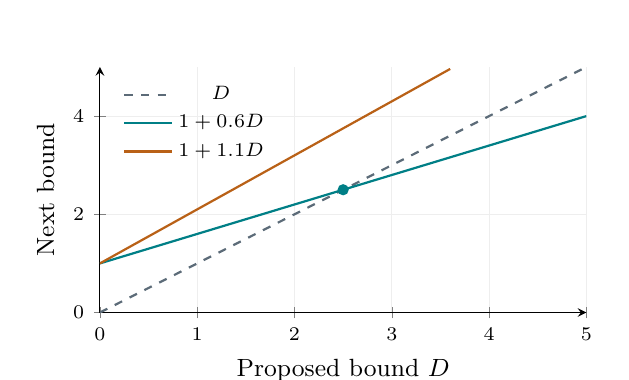
\begin{tikzpicture}
\begin{axis}[guide,width=.64\linewidth,height=47mm,xmin=0,xmax=5,ymin=0,ymax=5,xlabel={Proposed bound $D$},ylabel={Next bound},legend pos=north west]
\addplot[muted,dashed,domain=0:5] {x};\addlegendentry{$D$}
\addplot[teal,domain=0:5] {1+.6*x};\addlegendentry{$1+0.6D$}
\addplot[orange,domain=0:3.6] {1+1.1*x};\addlegendentry{$1+1.1D$}
\addplot[only marks,teal] coordinates{(2.5,2.5)};
\end{axis}
\end{tikzpicture}
\end{center}
\captext{Illustration with $F=1$. When $q_{\rm fb}=0.6$, the invariant bound is
$D=2.5$. When $q_{\rm fb}=1.1$, no nonnegative $D$ solves
$D\ge1+1.1D$. Making $\al_k$ smaller cannot fix that coefficient.}

\chapterpage{10}{Transfer to the paper's target}{Expectation cancels the linear term}
A high-probability bound around $S_\phi^{(k)}$ does not by itself control
the deterministic target $S_{\rm pdf}^{(k)}$.
We need the \emph{expected score} of the actual residual at $S_\phi^{(k)}$.
Using $Y^{(k)}=X_\phi^{(k)}+\eps-E_k$, Taylor expansion gives
\begin{align*}
 |\text{expected score at }S_\phi^{(k)}|
 \le{}&\left|\sum_u a_{tu}^{(k)}\E[g_{ktu}\Lambda_k(u)]\right|\\
 &+L_2\E\norm{\Theta_k}_\infty
       +\frac{L_3}{2}\E\norm{E_k}_\infty^2.
\end{align*}
The potentially first-order term is the first line. Expand
$\Lambda_k(u)=\sum_v\gamma_{uv}(\eps_v)$:
\begin{targetbox}
\[
 \E[g_{ktu}(\eps_u)\gamma_{uv}(\eps_v)]=0\quad(u\ne v).
\]
Independence separates the expectation and $\E\gamma_{uv}=0$.
Only the diagonal survives, and its weighted sum is at most
$L_2G_\infty\al_{k-1}$. That is the required second-order cancellation.
\end{targetbox}

\sub{Account for the exceptional event}
The high-probability estimates hold only while $z\bar\al\le\eta$.
Set $z_0=\log(10nK)$ and $x_* =\eta/\bar\al-z_0>0$.
Assume $\mu_4=\E|\eps|^4<\infty$. Let $m_\rho$ solve
$\E\rho'(\eps-m_\rho)=0$ and set
\[
 M_4=2^{K+1}\{\norm X_\infty+(n\mu_4)^{1/4}+|m_\rho|\}.
\]
Integrate the tail bounds up to $x_*$. Control the remaining expectation
by Cauchy--Schwarz and the fourth moment. This gives
\begin{align*}
 \E\norm{\Theta_k}_\infty&\le U_k
 =D\al_{k-1}(z_0+1)+(M_4+C_BK/\lambda)e^{-x_*/2},\\
 \E\norm{E_k}_\infty^2&\le W_k
 =A^2\al_{k-1}(z_0+1)+M_4^2e^{-x_*/2}.
\end{align*}
Here $W_k$ is a scalar moment bound, called $V_k^{\rm mom}$ in the
technical note. It is not a smoothing matrix.

\sub{Turn score error into location error}
Define
\[
 \beta_k=L_2G_\infty\al_{k-1}+L_2U_k+(L_3/2)W_k.
\]
If $L_3\sqrt{W_k}\le\lambda/4$ and $\beta_k\le\lambda^2/(8L_3)$,
the population score has slope magnitude at least $\lambda/2$ near its
zero. The same root argument as page 4 yields
\begin{targetbox}
\[
 \norm{S_{\rm pdf}^{(k)}-S_\phi^{(k)}}_\infty\le2\beta_k/\lambda.
\]
If both exponential tail terms above are at most
$\al_{\min}=\min_j\al_j$, then $\beta_k=O((z_0+1)\al_{k-1})$.
The target correction is second order. At stage one it is exactly zero.
\end{targetbox}

\chapterpage{11}{The theorem, with its conditions visible}{What has been proved}
Assume deterministic normalized weights, independent identically distributed
noise, the smoothed absolute loss, and the following fixed bounds:
\[
 f_{kt}\ge\lambda>0,\quad
 \al_j\le C_\al\al_k a^{-(k-j)},\quad
 \norm{B_{m:l}}_\infty\le C_B,\quad
 d<\frac{a-1}{C_BC_\al}.
\]
All indices range over the finite grid and stages $1,\ldots,K$.
Choose $\delta$, $A$, $D$ as on page 9. The sample-size requirement is
$z\bar\al\le\eta$, where
\[
 \eta=\min\left\{1,
 \left(\frac{\lambda}{4L_2c_v^*}\right)^2,
 \left(\frac{\lambda^2}{8L_3c_u^*}\right)^2,
 \left(\frac{\delta-d}{b_0c_v^*}\right)^2,
 \left(\frac{A_\Lambda}{D}\right)^2\right\}.
\]
The five entries respectively ensure the Bernstein simplification, local
curvature, local root control, small curvature fluctuation, and induction
localization. None assumes a bound on an unknown recursive remainder.

\begin{idea}
\textbf{Simultaneously for all $k\le K$, with probability at least $1-e^{-x}$,}
\begin{align*}
 \norm{\Theta_{k+1}}_\infty&\le Dz\al_k,\\
 \norm{\Phi_k}_\infty&\le\{P(A)+\delta Dr\}z\al_k,\\
 \norm{\widetilde S^{(k)}-S_\phi^{(k)}}_\infty
       &\le A_\Lambda\sqrt{z\al_k}+D(1+r)z\al_k.
\end{align*}
Add the fourth-moment and localization conditions on page 10 to obtain
\[
 \norm{\widetilde S^{(k)}-S_{\rm pdf}^{(k)}}_\infty
 \le A_\Lambda\sqrt{z\al_k}+D(1+r)z\al_k+2\beta_k/\lambda.
\]
With the stated tail control and $\al_k\asymp(nh_k)^{-1}$, this is
$A_1\sqrt{z/(nh_k)}+A_2z/(nh_k)$, with constants uniform in the stage
when the assumed parameters and dispersion margin are uniform.
\end{idea}

\sub{An explicit regime where all conditions eventually hold}
Take a constant signal, Gaussian noise $N(0,\sigma^2)$, $H=2\sigma$, and
nested block averages. Each stage halves the block size:
\begin{center}
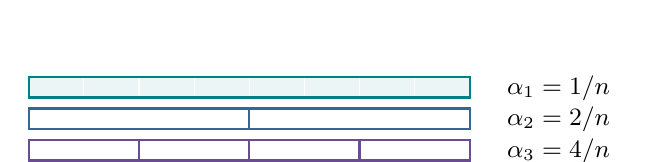
\begin{tikzpicture}[x=.7cm,y=.4cm]
\foreach \j in {0,...,7}{\draw[fill=teal!8,draw=white] (\j,2) rectangle ++(1,.65);}
\draw[thick,teal] (0,2) rectangle (8,2.65);
\draw[thick,blue] (0,1) rectangle (4,1.65);\draw[thick,blue] (4,1) rectangle (8,1.65);
\foreach \j in {0,2,4,6}{\draw[thick,purple] (\j,0) rectangle ++(2,.65);}
\node[anchor=west,font=\small] at (8.5,2.3) {$\al_1=1/n$};
\node[anchor=west,font=\small] at (8.5,1.3) {$\al_2=2/n$};
\node[anchor=west,font=\small] at (8.5,.3) {$\al_3=4/n$};
\end{tikzpicture}
\end{center}
Here $a=2$, $C_\al=1$, $C_B=2$, and
$d\le\sqrt{1.25/\sqrt{1.5}-1}\approx0.144<1/2$.
For $K\le c\log_2n$ with fixed $0<c<1$,
$z\bar\al=O(n^{c-1}\log n)\to0$.
The moment tails decay faster than any polynomial, so the target conditions
also hold eventually. This proves that the sufficient conditions describe
a nonempty regime with a growing number of components.
\captext{This example uses nested block weights. It does not certify the
convolution windows in the archive.}

\chapterpage{12}{What the archive shows, and what it does not}{Read the evidence correctly}
The archive's Monte Carlo runs measure how closely the leading term
$L_k$ approximates the actual error $e_k$ relative to $S_\phi^{(k)}$.
The plotted quantity is the median of $\norm{e_k-L_k}_\infty/\norm{e_k}_\infty$.

\begin{center}
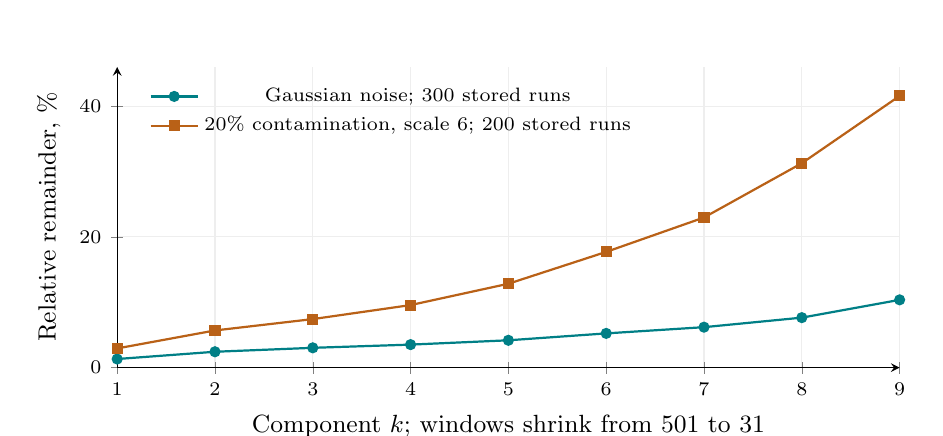
\begin{tikzpicture}
\begin{axis}[guide,width=.95\linewidth,height=54mm,xmin=1,xmax=9,ymin=0,ymax=46,xtick={1,...,9},xlabel={Component $k$; windows shrink from 501 to 31},ylabel={Relative remainder, \%},legend pos=north west]
\addplot[teal,mark=*] coordinates {\mcGaussian};\addlegendentry{Gaussian noise; 300 stored runs}
\addplot[orange,mark=square*] coordinates {\mcContaminated};\addlegendentry{20\% contamination, scale 6; 200 stored runs}
\end{axis}
\end{tikzpicture}
\end{center}
\captext{Stored archive results. Contamination adds a random-sign exponential outlier
with mean magnitude $6\sigma$ at 20\% of points. These medians do not measure theorem failure probabilities.}

\sub{Apply the new sufficient conditions to the Gaussian design}
For $n=1000$, $H=0.8$, $\sigma=0.4$ and the nine archive windows,
the floating-point checks at 95\% confidence give:
\begin{center}
\renewcommand{\arraystretch}{1.22}
\begin{tabular}{@{}p{60mm}p{61mm}l@{}}
\toprule
Condition & Calculated comparison & Outcome\\
\midrule
Curvature dispersion & $0.17112<0.19517$ & \textcolor{teal}{passes}\\
Feedback coefficient & $q_{\rm fb}\approx0.93838<1$ & \textcolor{teal}{passes}\\
Finest-scale requirement & $1.4371\le3.9993\times10^{-10}$ & \textcolor{orange}{fails}\\
\bottomrule
\end{tabular}
\end{center}
The induction constant is about $1.45\times10^6$. Its localization
requirement dominates $\eta$. The theorem is therefore far too conservative
to certify these runs. Improving constants or finding a sharper propagation
argument is a separate task; the empirical agreement does not remove that gap.

\begin{idea}
\textbf{Five checks to carry away}
\begin{enumerate}
\item Can a stage use fresh-noise concentration? No. Group by original observation.
\item Is $\Phi_k$ a single-pass error? No. It measures the effect of earlier errors on the next input.
\item Why is $Z_k\Lambda_k$ second order? Off-diagonal centering, plus a separately bounded diagonal.
\item What closes the induction? A fixed $A$, a coefficient $q_{\rm fb}<1$, and $D=F/(1-q_{\rm fb})$.
\item Why are the targets close? Cancellation of the expected linear term, followed by moment and curvature control.
\end{enumerate}
\end{idea}

\sub{Where to find the full derivations}
\small
The companion \href{../irmf_all_components_bound.pdf}{\textit{Bounds for all recursive IRMF components}}
contains the full proofs and explicit constants. The
\href{../irmf_recursive_component_bounds.pdf}{\textit{reviewed partial-results note}}
contains the Fourier and perturbation arguments.
Plot coordinates come from the archived audit results and
\texttt{build\_visual\_guide.py}; the condition values come from
\texttt{all\_components\_conditions.json}.
This guide replaces the original tutorial's unsupported closure claims
with the restricted theorem and its actual applicability checks.
\end{document}
